\documentclass[a4paper,12pt]{article}

\usepackage[utf8]{inputenc}
\usepackage[danish]{babel}

\usepackage{todonotes}
\usepackage{float} % for [H]
\usepackage{listings}

\lstset{
  language=C,
  basicstyle=\ttfamily,
  columns=fullflexible,
  showstringspaces=false,
  commentstyle=\color{gray}\upshape,
  basicstyle=\small,
  numberstyle=\footnotesize,
  numbers=left,
  captionpos=b,
  stepnumber=1,
  numbersep=10pt,
  tabsize=4,
  breaklines=true,
  morekeywords={bool}
}

\title{Test and Verification: Verification Miniproject}
\author{Jesper Riemer Andersen: 20102569\\Simon Reedtz Olesen: 20102589}

\begin{document}
\maketitle

\begin{figure}[H]
\centering
\includegraphics[width=0.8\linewidth]{Crossing_The_River.png}
\caption{Crossing the river}
\end{figure}

\begin{lstlisting}
bool canInflictViolence()
{
    return canMomInflictViolence() || canDadInflictViolence() || canThiefInflictViolence();
}
\end{lstlisting}

\begin{figure}[H]
\centering
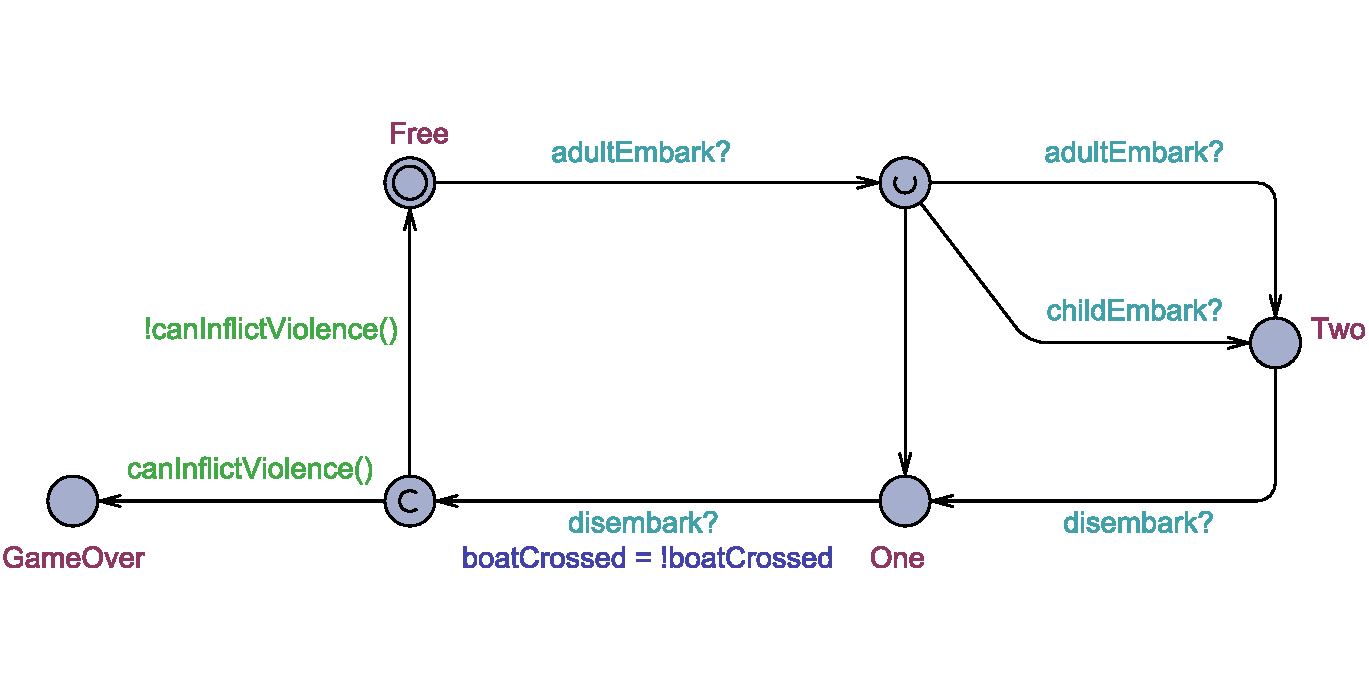
\includegraphics[width=\linewidth]{Boat.pdf}
\caption{Crossing the river}
\end{figure}

\begin{figure}[H]
\centering
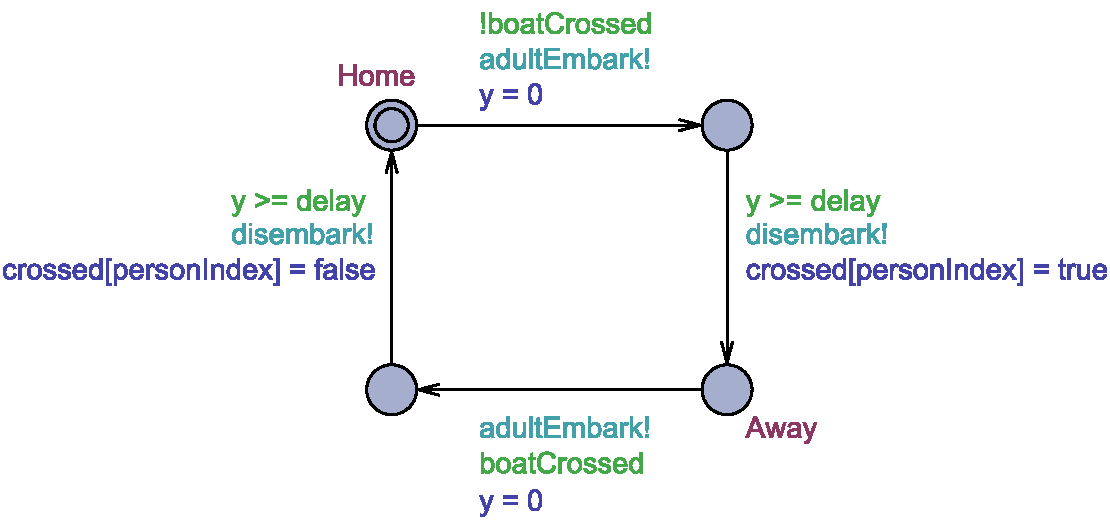
\includegraphics[width=\linewidth]{Adult.pdf}
\caption{Crossing the river}
\end{figure}

\begin{figure}[H]
\centering
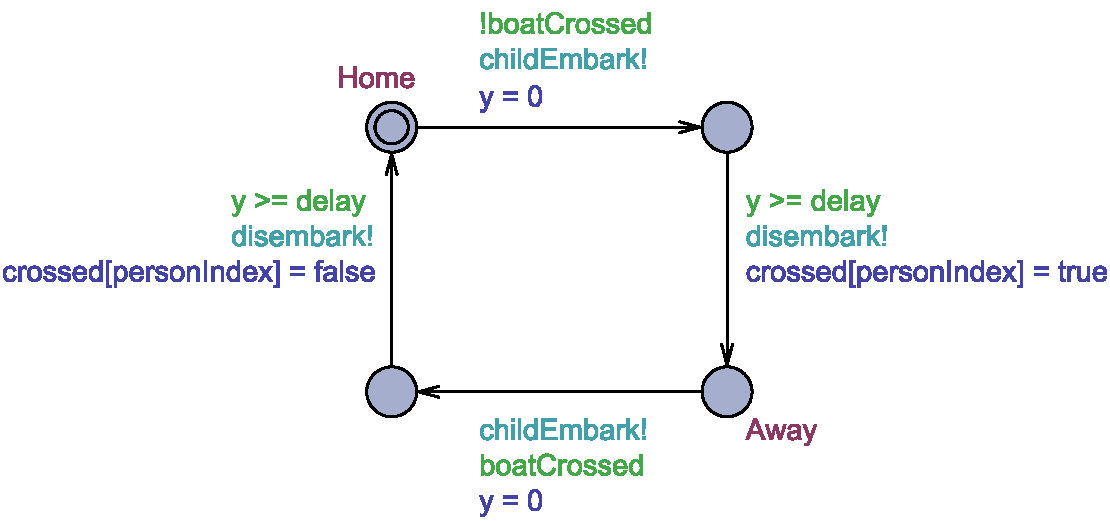
\includegraphics[width=\linewidth]{Child.pdf}
\caption{Crossing the river}
\end{figure}

\end{document}